% ============================================================
% HPC-Accelerated Automated Workflow for Virtual Screening
% Target: Wiley Applied Research (ISSN 2702-4288)
% Format: Wiley NJD-compatible, numbered references
% ============================================================
\documentclass[11pt,a4paper]{article}

% --- Core packages ---
\usepackage[margin=2.5cm]{geometry}
\usepackage[T1]{fontenc}
\usepackage{lmodern}
\usepackage{microtype}
\usepackage[utf8]{inputenc}

% --- Math & symbols ---
\usepackage{amsmath,amssymb}

% --- Graphics & tables ---
\usepackage{graphicx}
\graphicspath{{figures/}}
\usepackage{booktabs}
\usepackage{longtable}
\usepackage{multirow}
\usepackage{array}
\usepackage{tabularx}

% --- Chemistry & units ---
\usepackage{textcomp}
\usepackage{siunitx}
\sisetup{detect-all, group-separator={,}}

% --- Bibliography (numbered, Wiley Chemistry-Materials style) ---
\usepackage[numbers,sort&compress]{natbib}
\renewcommand{\bibnumfmt}[1]{#1.}

% --- Hyperlinks ---
\usepackage{xcolor}
\usepackage[colorlinks=true,linkcolor=blue!60!black,citecolor=blue!60!black,urlcolor=blue!60!black]{hyperref}

% --- Line numbering (for review) ---
\usepackage{lineno}
\linenumbers

% --- Captions ---
\usepackage[font=small,labelfont=bf]{caption}

% --- Headers ---
\usepackage{fancyhdr}
\pagestyle{fancy}
\fancyhf{}
\fancyhead[L]{\small\textit{Applied Research} --- Manuscript}
\fancyhead[R]{\small\thepage}
\renewcommand{\headrulewidth}{0.4pt}

% --- Author block formatting ---
\usepackage{authblk}
\renewcommand\Authfont{\normalsize\bfseries}
\renewcommand\Affilfont{\small\normalfont}

% --- Section formatting ---
\usepackage{titlesec}
\titleformat{\section}{\large\bfseries}{\thesection.}{0.5em}{}
\titleformat{\subsection}{\normalsize\bfseries}{\thesubsection}{0.5em}{}
\titleformat{\subsubsection}{\normalsize\itshape}{\thesubsubsection}{0.5em}{}

% --- Double spacing for review ---
\usepackage{setspace}
\doublespacing

% ============================================================
\begin{document}

% ============================================================
% TITLE
% ============================================================
\title{\textbf{Design and Benchmarking of an HPC-Accelerated Automated Workflow for Virtual Screening of Thai Traditional Herbal Asthma Formulations}}

\author[1]{Ratchaneekorn Weerasin}
\author[1]{Worawan Marurngsith}
\author[2]{Neal M.\ Davies}
\author[3]{Phuphiphat Jaikaew}
\author[4,*]{Kewalin Inthanon}

\affil[1]{Department of Computer Science, Faculty of Science and Technology, Thammasat University, Lampang Campus, Thailand}
\affil[2]{Faculty of Pharmacy \& Pharmaceutical Sciences, University of Alberta, Canada}
\affil[3]{Department of Biotechnology, Faculty of Science and Technology, Thammasat University, Rangsit Campus, Thailand}
\affil[4]{Department of Biotechnology, Faculty of Science and Technology, Thammasat University, Lampang Campus, Thailand}

\date{}

\maketitle
\thispagestyle{fancy}

\noindent\textbf{*Corresponding author:} Kewalin Inthanon, Department of Biotechnology, Faculty of Science and Technology, Thammasat University, Lampang Campus, Thailand. Email: \href{mailto:inthanon@tu.ac.th}{inthanon@tu.ac.th}

% ============================================================
% ABSTRACT
% ============================================================
\begin{abstract}
\noindent
The multi-component nature of traditional herbal formulations poses a significant challenge for computational drug discovery, as multiple phytochemicals simultaneously interact with various biological targets. This combinatorial complexity generates large docking matrices that demand substantial computational resources. We present a high-performance computing (HPC)-accelerated automated workflow for multi-target virtual screening, validated on a Thai traditional anti-asthma polyherbal formulation containing \textit{Aloe vera}, \textit{Cocos nucifera}, \textit{Solanum xanthocarpum}, and \textit{Zingiber montanum}. The workflow achieved a \SI{92.9}{\percent} data reduction through bioinformatics filtering, prioritizing 14 protein targets from 197 raw predictions. Benchmarking on the LANTA supercomputer demonstrated a 118.59-fold practical speedup, reducing the wall-clock time for 126 docking pairs from \SI{8.4}{hours} (sequential, workstation) to \SI{4.25}{minutes} (parallel, HPC), with throughput increasing from 15 to 1,779~docking~jobs/hour. Parallel efficiency reached \SI{94.12}{\percent} with high numerical fidelity ($r = 0.9974$). Scalability projections indicated feasibility for datasets of up to $10^6$ docking pairs. The case study identified solasodine as a promising candidate with strong predicted binding to PTGS2 (COX-2) and ALDH1A1. The workflow architecture, benchmarking methodology, and scalability analysis provide a reusable framework for HPC-accelerated virtual screening of multi-component natural product formulations.
\end{abstract}

\noindent\textbf{Keywords:} high-performance computing; parallel execution; automated workflow; molecular docking; LANTA supercomputer; Thai traditional medicine; virtual screening

% ============================================================
% 1. INTRODUCTION
% ============================================================
\section{Introduction}

Herbal medicines typically contain combinations of various plant extracts with diverse phytochemicals. From a computational systems biology perspective, this represents a multi-component, multi-target pharmacological model that produces a combinatorial matrix of ligand--target interactions. Even a simple polyherbal formulation generates hundreds or thousands of possible ligand--protein docking events. This combinatorial effect constitutes a major challenge for computational analysis, as conventional sequential docking rapidly becomes computationally expensive and difficult to scale for systematic screening \cite{jeyasingh2024,babalola2025}.

In this research, asthma serves as an exceptionally relevant disease paradigm for studying multi-target pharmacology. Asthma is a multifactorial respiratory disease involving complex inflammatory signaling cascades, immune regulation, airway remodeling, and bronchial hyperresponsiveness \cite{gina2023,vos2020}. Because multiple molecular pathways are implicated in disease progression, therapeutic approaches often involve modulation of multiple biological targets rather than a single molecular mechanism. This biological complexity aligns well with the multi-component nature of herbal medicines, which may exert pharmacological effects through coordinated modulation of multiple signaling pathways.

Modern computer-aided drug discovery (CADD) workflows are inherently multi-stage and data-intensive \cite{siddiqui2025,gupta2024}. A typical workflow consists of automated compound retrieval from PubChem via the REST API, compound standardization using SMILES representations, target prediction via ChEMBL, KEGG pathway analysis, ligand force field optimization, protonation normalization, protein preparation, grid parameterization, and result aggregation. Each step generates intermediate data that must be retained for traceability and reproducibility. As dataset size increases, both filesystem pressure and computational load grow proportionally, often leading to I/O bottlenecks that degrade practical throughput despite nominal hardware capability \cite{roy2024}.

Although large-scale frameworks such as VirtualFlow have successfully handled billion-scale docking campaigns, these systems require highly specialized infrastructure and complex configuration \cite{gorgulla2020,gorgulla2023}. In addition, large numbers of small intermediate files introduce scheduler overhead and metadata contention in shared parallel filesystems. For multi-target herbal screening, where flexibility and reproducibility are critical, such ultra-large screening frameworks may not provide optimal architectural efficiency.

Molecular docking is an inherently embarrassingly parallel problem: each ligand--protein pair can be evaluated independently without inter-task communication. This property makes it suitable for high-performance computing (HPC) environments. However, achieving efficient scalability requires careful attention to CPU-core-to-task mapping, batch size management to balance scheduler efficiency and queue latency, and file I/O management to avoid filesystem contention. Without these optimizations, parallel execution risks diminishing returns due to scheduler dispatch latency and filesystem contention \cite{chowdhury2020}.

In Thailand, the LANTA supercomputer employs a multi-node CPU architecture and the SLURM workload manager for resource management \cite{varavithya2023}. SLURM job arrays enable structured execution of independent molecular docking tasks, providing deterministic mapping of ligand--protein pairs to individual CPU cores while maintaining centralized resource allocation control \cite{goponenko2024}. However, infrastructure alone is insufficient to ensure execution efficiency. A reproducible and automated end-to-end workflow is essential to integrate database mining, target filtering, structure preprocessing, parallel execution, and post-processing aggregation within a unified computational framework.

The objective of this research is to design, develop, and benchmark an HPC-accelerated automated workflow optimized for natural product-based multi-target screening. The contribution lies not in developing a new docking tool but in workflow engineering that incorporates automatic compound and target collection from PubChem, ChEMBL, and KEGG databases; Boolean classification-based target reduction; ligand--protein preprocessing standardization; and SLURM job array management with controlled CPU core allocation. Performance benchmarking encompasses wall-clock time reduction, throughput scaling, parallel efficiency, scheduler latency, and numerical reproducibility relative to sequential execution.

The principal contributions of this work are threefold: (i)~an end-to-end automated workflow that integrates heterogeneous bioinformatics databases with HPC-accelerated molecular docking; (ii)~a systematic performance benchmarking methodology, including speedup, parallel efficiency, throughput, and numerical reproducibility metrics, evaluated on the LANTA supercomputer; and (iii)~a scalability analysis demonstrating the feasibility of extending the workflow from ethnopharmacological-scale datasets to high-throughput screening libraries of $10^6$ compounds.

To validate the workflow, a case study on a Thai traditional anti-asthma polyherbal formulation was conducted. Phytochemical--target interactions were systematically evaluated through molecular docking and benchmarking against standard asthma drugs. By emphasizing orchestration efficiency, file management stability, and scalability under realistic HPC constraints, this research establishes a computational platform for multi-component herbal screening.


% ============================================================
% 2. METHODOLOGY
% ============================================================
\section{Methodology}

\subsection{Overview of the HPC-accelerated automated workflow}

The overall architecture of the HPC-accelerated automated workflow is presented in Figure~\ref{fig:workflow}. The virtual screening workflow was designed as a three-phase computational framework integrating data acquisition, target prioritization, and high-performance molecular docking. Phase~I focused on phytochemical data collection. Phase~II included target prediction and pathway-based prioritization to identify asthma-related protein targets. Phase~III involved large-scale molecular docking using the AutoDock Vina engine on the LANTA supercomputer via SLURM job arrays, followed by interaction profiling and result aggregation.

\subsection{Databases, software, and computational tools}

The databases and software libraries employed in this research are summarized below. PubChem (\url{https://pubchem.ncbi.nlm.nih.gov/}), ChEMBL (\url{https://www.ebi.ac.uk/chembl/}), Google Scholar, PubMed, SwissTargetPrediction (\url{http://www.swisstargetprediction.ch/}), KEGG (\url{https://www.genome.jp/kegg/pathway.html}), and the RCSB Protein Data Bank (PDB; \url{https://www.rcsb.org/}) were used for data retrieval. Computational analyses were performed using Python~3.13.5 with associated libraries: RDKit~2025.03.6, Open Babel~3.1.1 \cite{oboyle2011}, NetworkX~3.3 \cite{hagberg2008}, Matplotlib~3.9.2 \cite{hunter2007}, and BioPython~1.85. Environment management used Conda~25.7.0. Molecular docking was performed using AutoDock Vina~1.1.2 \cite{seeliger2010}. HPC computations were executed on the LANTA supercomputer with SLURM~24.05 \cite{jette2023}. Docking poses were visualized using PyMOL~3.1.6.1.

\begin{figure}[!ht]
\centering
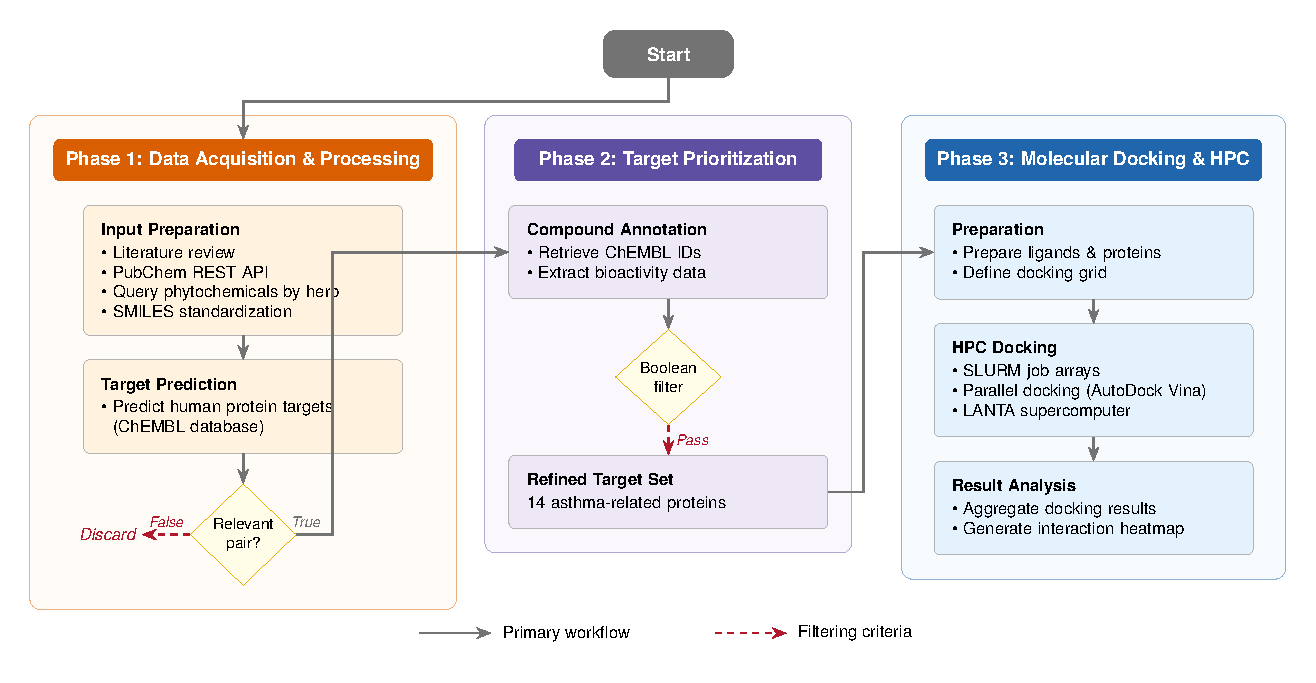
\includegraphics[width=\textwidth]{fig1_workflow.pdf}
\caption{Overview of the HPC-accelerated automated workflow for multi-target virtual screening of phytochemicals in a Thai traditional anti-asthma formulation.}
\label{fig:workflow}
\end{figure}


\subsection{Computational environment and hardware specification}

Two computational environments were used to assess the performance and scalability of the proposed workflow.

\subsubsection{Sequential baseline environment (workstation)}

A mobile workstation was used with an AMD Ryzen\textsuperscript{\texttrademark}~5 7535HS processor (6~cores/12~threads, Zen~3+, boost clock \SI{4.55}{GHz}) and \SI{16}{GB} DDR5-4800 memory. Network connectivity was provided via Wi-Fi~6 (2$\times$2 AX).

\subsubsection{HPC environment (LANTA)}

HPC operations were carried out on the LANTA supercomputer. Each compute node was equipped with dual AMD EPYC~7543 processors (64~physical cores per node, Zen~3 Milan architecture, max boost clock \SI{2.8}{GHz}) and \SI{256}{GB} system memory. Nodes were interconnected via Slingshot-11 HSN at \SI{200}{Gbps}, equivalent to HDR InfiniBand.


\subsection{Phytochemical data acquisition (Phase~I)}

An automated workflow was developed for the integrated retrieval and prioritization of phytochemical compound and asthma-related gene information.

\subsubsection{Phytochemical--compound mapping and data acquisition}

The phytochemical constituents of four medicinal herbs commonly employed in Thai anti-asthma formulations---\textit{Aloe vera}, \textit{Cocos nucifera}, \textit{Solanum xanthocarpum}, and \textit{Zingiber montanum}---were systematically compiled through literature review and public database mining. Chemical identity and bioactivity information related to asthma or inflammation was collected from Google Scholar, PubMed, and PubChem. For each compound, an automated Python-based workflow queried the PubChem REST API to extract the Compound ID (CID) and canonical SMILES representation. The SMILES of each compound was then used to retrieve its associated ChEMBL ID via an automated API query. Human protein targets for each compound were obtained from ChEMBL and matched with their corresponding gene symbols.

\subsubsection{Integration of asthma gene set from KEGG}

An asthma-related gene set was downloaded using the KEGG REST API from the KEGG asthma pathway. All genes were standardized for subsequent comparative analysis. Predicted human target genes for each compound were compared with the KEGG-derived asthma gene set.

\subsubsection{Boolean classification logic}

A Python function, \texttt{analyze\_compound}, was created to perform set intersection analysis between predicted compound targets and the KEGG-derived asthma gene set. Compounds were classified as \emph{relevant}~(True) if at least one predicted target overlapped with the asthma gene set, or \emph{non-relevant}~(False) otherwise. For relevant compounds, the matched genes were recorded and stored. Results were appended to structured data objects iteratively. After all compound iterations, the aggregated dataset---including compound IDs, predicted targets, overlap status, and matched genes---was exported in CSV format for reproducibility.

\subsubsection{Data reduction ratio}

The filtration efficiency was quantified using the Data Reduction Ratio (DRR) \cite{awan2016}:
%
\begin{equation}
\text{DRR} (\%) = \left(1 - \frac{N_{\text{filtered}}}{N_{\text{initial}}}\right) \times 100
\label{eq:drr}
\end{equation}
%
where $N_{\text{initial}}$ is the total number of predicted phytochemical--protein interactions prior to filtering and $N_{\text{filtered}}$ is the number of biologically relevant targets retained after Boolean classification and pathway-based filtering.


\subsection{Pathway-based filtering and final target selection (Phase~II)}

Initial target predictions from Phase~I were refined through pathway-focused filtering. SwissTargetPrediction \cite{daina2019} was employed to enrich the target list obtained from ChEMBL. Chemical similarity and known ligand--target pairs were used for enrichment. The predicted target list was then linked to KEGG pathways via the KEGG REST API. Only protein targets involved in asthma- and inflammation-related pathways were retained.

Relationships between compounds, targets, and pathways were visualized using NetworkX \cite{hagberg2008} and Matplotlib \cite{hunter2007} to identify key proteins in the interaction network. Final target prioritization was based on: (i)~consistency of predicted targets across compound screening and KEGG pathway mapping; (ii)~literature-based relevance to asthma pathophysiology; and (iii)~biological plausibility based on protein mechanisms of action. Only targets with crystal structures deposited in the PDB at resolution $\leq$~3~\AA{} were selected \cite{flachsenberg2023}. Preference was given to structures co-crystallized with ligands.


\subsection{Molecular docking workflow implementation (Phase~III)}

The molecular docking workflow was designed as a standardized and reproducible computational module comprising ligand preprocessing, protein preprocessing, docking parameter configuration, and grid standardization.

\subsubsection{Ligand preparation}

Three-dimensional ligand structures were downloaded from PubChem in SDF format. Preprocessing was performed using RDKit and Open Babel \cite{oboyle2011} and included: (i)~addition of hydrogen atoms, (ii)~geometry optimization using the MMFF94 force field as implemented in RDKit, and (iii)~protonation state adjustment at physiological pH~7.4. Preprocessed ligands were converted to PDBQT format.

\subsubsection{Protein preparation}

Crystal structures for the protein targets were retrieved from the Protein Data Bank. Protein structures were preprocessed using custom Python scripts and the Biopython library. Preprocessing steps included: (i)~removal of crystallographic water molecules and non-essential heteroatoms, (ii)~addition of polar hydrogens, (iii)~assignment of Gasteiger charges \cite{gasteiger1980}, and (iv)~retention of the protein backbone as rigid bodies. Structures were exported in PDBQT format for docking simulations.

\subsubsection{Docking configuration and grid standardization}

Molecular docking was performed using AutoDock Vina~1.1.2 \cite{seeliger2010}. The following parameters were standardized across all simulations: exhaustiveness~=~8, number of output modes~=~9, and energy range~=~\SI{3}{kcal/mol}. Grid maps were generated to encompass the active sites of each protein target. Where available, grid centers were aligned with co-crystallized ligand positions. Grid dimensions were kept consistent to minimize parameter variation between sequential and HPC simulations. Identical configuration files were used for both execution modes.


\subsection{HPC architecture}

The parallel computing architecture is shown in Figure~\ref{fig:hpc-arch}. All large-scale docking simulations were performed on the LANTA system through the SLURM workload manager. The HPC cluster consisted of multiple compute nodes equipped with multi-core CPUs connected through high-speed interconnects. SLURM managed job scheduling and resource allocation, distributing computational tasks to available compute nodes.

\begin{figure}[!ht]
\centering
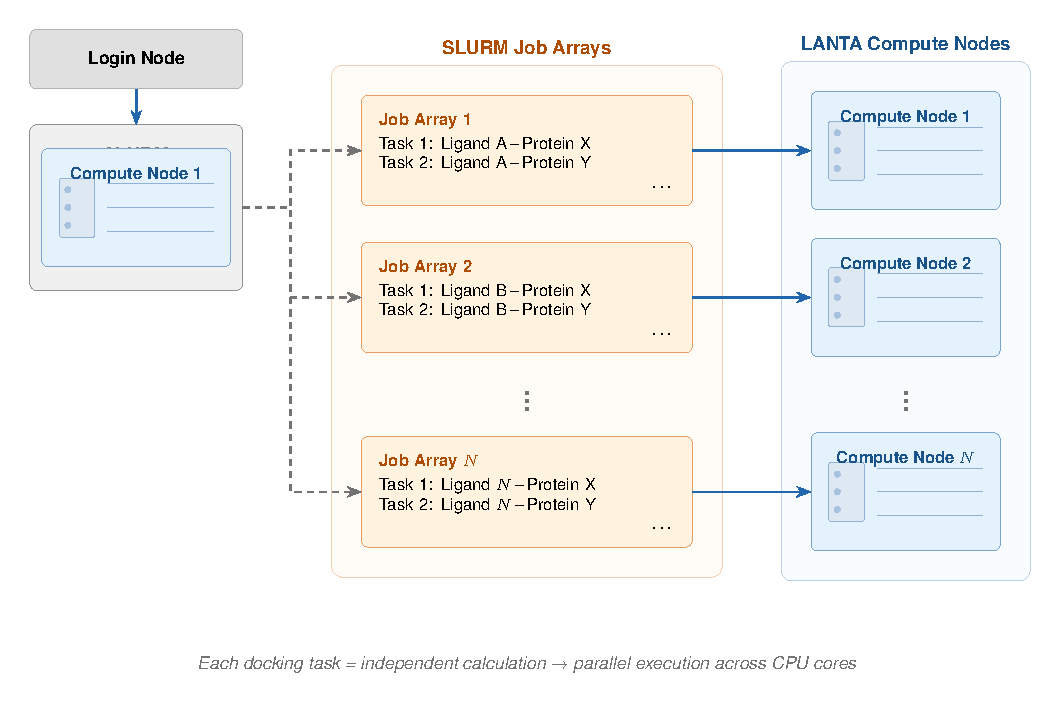
\includegraphics[width=\textwidth]{fig2_hpc_architecture.pdf}
\caption{Architecture of the HPC execution framework for large-scale molecular docking on the LANTA supercomputer.}
\label{fig:hpc-arch}
\end{figure}


\subsection{Parallel execution strategy}

To accelerate large-scale docking computations, task-level parallelization was executed on the LANTA supercomputer using the SLURM workload manager~(version~24.05) \cite{jette2023}. Each ligand--target pair was treated as an independent computational task. In total, 126~tasks were executed, corresponding to 9~ligands~$\times$~14~targets. Tasks were distributed across CPU cores using the SLURM job array command (\texttt{-{}-array=1-126}).


\subsection{Performance metrics and validation}

The HPC-accelerated workflow was evaluated using the following performance metrics.

\subsubsection{Wall-clock execution time}

Wall-clock time ($T$) is the total elapsed time from job submission to final output generation. Two execution modes were compared: $T_{\text{seq}}$ (sequential workflow) and $T_{\text{HPC}}$ (HPC-accelerated workflow). All time measurements were recorded from system logs.

\subsubsection{Speedup}

Computational acceleration from parallel processing was measured as the speedup factor \cite{amdahl1967}:
%
\begin{equation}
S = \frac{T_{\text{seq}}}{T_{\text{HPC}}}
\label{eq:speedup}
\end{equation}
%
A speedup $S > 1$ indicates improved performance through parallelization. For embarrassingly parallel workloads with negligible inter-task communication, the theoretical maximum speedup approaches $N$ (the number of processing units), corresponding to ideal linear scaling \cite{amdahl1967}.

\subsubsection{Parallel efficiency}

Parallel efficiency ($E$) measures the utilization of available computational resources \cite{eijkhout2010}:
%
\begin{equation}
E = \frac{S}{N}
\label{eq:efficiency}
\end{equation}
%
where $S$ is the speedup factor and $N$ is the number of CPU cores. An efficiency close to 1 indicates minimal overhead.

\subsubsection{Throughput}

Docking throughput ($\Theta$) quantifies the number of completed docking tasks per unit time:
%
\begin{equation}
\Theta = \frac{N_{\text{tasks}}}{T}
\label{eq:throughput}
\end{equation}
%
where $N_{\text{tasks}}$ is the total number of docking pairs (126) and $T$ is the wall-clock execution time in hours.

\subsubsection{Statistical validation of numerical consistency}

Binding affinity scores from the sequential and HPC workflows were compared using Pearson's correlation coefficient ($r$) \cite{hothorn2011} across all 126 docking pairs:
%
\begin{equation}
r = \frac{\sum_{i}(x_i - \bar{x})(y_i - \bar{y})}{\sqrt{\sum_{i}(x_i - \bar{x})^2 \sum_{i}(y_i - \bar{y})^2}}
\label{eq:pearson}
\end{equation}
%
where $x_i$ and $y_i$ represent docking scores from the sequential and HPC workflows, respectively, and $\bar{x}$ and $\bar{y}$ are the corresponding means.


\subsection{Scalability projection model}

To assess the scalability potential of the proposed workflow for large-scale virtual screening, a theoretical runtime estimation was performed using empirical performance data from LANTA.

\subsubsection{Projection model}

The estimation is based on the parallel efficiency ($E$) measured during benchmarking on 126~docking pairs. The projected time ($T_{\text{proj}}$) for a larger dataset is \cite{gorgulla2020}:
%
\begin{equation}
T_{\text{proj}} = \frac{N_{\text{pairs}} \times \bar{t}_{\text{seq}}}{N_{\text{cores}} \times E}
\label{eq:projection}
\end{equation}
%
where $N_{\text{pairs}}$ is the number of docking pairs in the expanded library (e.g., $10^6$), $\bar{t}_{\text{seq}}$ is the mean sequential execution time per pair (\SI{240}{s}), $N_{\text{cores}}$ is the number of parallel processing units, and $E$ is the observed parallel efficiency~(0.941).

\subsubsection{Assumptions and limitations}

This projection assumes that the embarrassingly parallel characteristic of molecular docking persists at scale, with assessment spanning from a small-scale ethnopharmacological dataset to high-throughput screening (HTS) scale of $10^6$~compounds. The analysis considers the AMD EPYC~7543 nodes' capacity for I/O operations and file management, facilitated by the automated Python-based preprocessing module. This assessment was carried out theoretically and was not tested in practice. In practice, SLURM job arrays are subject to system-configured limits (typically \texttt{MaxArraySize} of 1,001--10,001 tasks), and scaling to $10^6$ tasks would require array batching strategies and may encounter filesystem metadata contention on shared parallel filesystems.


\subsection{Comparative docking with standard asthma drugs}

To provide a clinical reference for interpreting binding affinity, two standard asthma drugs were selected as controls: dexamethasone (a corticosteroid with anti-inflammatory effects) and salbutamol (a $\beta_2$-adrenergic receptor agonist). Three-dimensional structures were obtained from PubChem and processed using the identical ligand preprocessing protocol outlined in Section~2.6.1. Binding affinities of phytochemical compounds were compared against these standard drugs.


% ============================================================
% 3. RESULTS
% ============================================================
\section{Results}

\subsection{Automated workflow validation}

The automated informatics workflow successfully processed nine phytochemicals from four medicinal plants in the Thai anti-asthma formulation (\textit{Aloe vera}, \textit{Cocos nucifera}, \textit{Solanum xanthocarpum}, and \textit{Zingiber montanum}). A total of 197~target proteins associated with 550~asthma-related pathways were retrieved from the KEGG database, underscoring the polypharmacological nature of traditional herbal formulations. The multi-target profile of phytochemicals is a recognized signature of natural products \cite{babalola2025}, particularly in asthma, a disease of considerable complexity involving immune, inflammatory, smooth muscle, and epithelial responses \cite{habib2022}.

Among the retrieved phytochemicals, emodin exhibited the largest interaction network with 113~associated protein targets and 237~pathways, whereas terpinen-4-ol demonstrated the fewest interactions. Phytochemical--target data are presented in Table~\ref{tab:phytochem}. Anthraquinones, including emodin, exhibit anti-inflammatory and immunomodulatory activities by modulating NF-$\kappa$B, MAPK, and arachidonic acid metabolism pathways \cite{habib2022,liu2026}. The wide predicted interaction network is consistent with existing literature characterizing emodin as a multi-target bioactive molecule \cite{liu2026}. Conversely, the limited predicted interactions for terpinen-4-ol may reflect the restricted scope of in-silico target prediction for small monoterpenes.

The KEGG-derived asthma-related targets were confirmed by Boolean classification, applying the condition that each compound interacted with at least one target. Fourteen asthma-related protein targets were identified following pathway-based refinement and validation through literature review (Table~\ref{tab:targets}). This functional diversity reflects the multifactorial pathophysiology of asthma, involving bronchoconstriction (ADRB2) \cite{slob2018}, inflammatory enzyme activity (PTGS2/COX-2) \cite{tanaka2024}, epigenetic regulation (HDAC6) \cite{potaczek2024}, metabolic reprogramming (FASN) \cite{ito2025}, and neurogenic inflammation (TRPV1) \cite{manti2024}.

\begin{table}[!ht]
\centering
\caption{Predicted protein targets and associated KEGG pathways for phytochemicals in the selected medicinal plants.}
\label{tab:phytochem}
\begin{tabular}{llcc}
\toprule
\textbf{Plant} & \textbf{Phytochemical} & \textbf{Predicted targets} & \textbf{KEGG pathways} \\
\midrule
\textit{Aloe vera}    & Emodin          & 113 & 237 \\
                       & Aloe-emodin     & 31  & 102 \\
                       & Aloin           & 4   & 13  \\
\textit{Cocos nucifera} & Lauric acid   & 24  & 97  \\
                       & Monolaurin      & 4   & 13  \\
\textit{S.\ xanthocarpum} & Solasodine  & 7   & 41  \\
\textit{Z.\ montanum}  & DMPBD          & 5   & 32  \\
                       & Sabinene        & 4   & 13  \\
                       & Terpinen-4-ol   & 5   & 2   \\
\bottomrule
\end{tabular}
\end{table}

\begin{table}[!ht]
\centering
\caption{Fourteen prioritized protein targets for anti-asthma phytochemicals, grouped by functional class with representative KEGG pathways.}
\label{tab:targets}
\small
\begin{tabularx}{\textwidth}{lp{3.5cm}X}
\toprule
\textbf{Functional group} & \textbf{Targets} & \textbf{Representative KEGG pathways} \\
\midrule
GPCRs & ADRB2, ADRA2A & Adrenergic signaling; Neuroactive ligand--receptor interaction; Inflammatory mediator regulation \\
Nuclear receptors & AR, ESR1, THRB, NR1C2 & Estrogen signaling; Thyroid hormone signaling; Steroid hormone-mediated signaling \\
Enzymes & PTGS2, HDAC6, ALDH1A1, FASN, ELANE, POLK, UGT2B7 & Arachidonic acid metabolism; Histone modification; Xenobiotic metabolism; Neutrophil degranulation \\
Ion channels & TRPV1 & TRP channel regulation; Neuroinflammation pathways \\
\bottomrule
\end{tabularx}
\end{table}

The automated workflow achieved a significant reduction in data volume. Through Boolean intersection with the KEGG-derived asthma target set, predicted interactions were reduced to a refined matrix of 14~protein targets, representing a \SI{92.9}{\percent} DRR. The workflow effectively isolated \SI{7.1}{\percent} of the original interaction landscape. This filtration is crucial to improve the signal-to-noise ratio and enables strategic allocation of HPC resources to mechanistically relevant targets rather than exploratory noise \cite{gorgulla2023,kotev2023}. The integrated compound--target--pathway network (Figure~\ref{fig:network}) demonstrates cross-talk among compounds, targets, and asthma-related KEGG pathways. Network-based approaches have been increasingly recommended for traditional medicine research, where therapeutic effects often arise from synergistic multi-component, multi-target interactions \cite{noor2022,yang2025}.

The output from this validation step confirmed that the HPC-automated workflow can consolidate heterogeneous phytochemical data into a biologically focused docking matrix suitable for high-throughput computational benchmarking.

\begin{figure}[!ht]
\centering
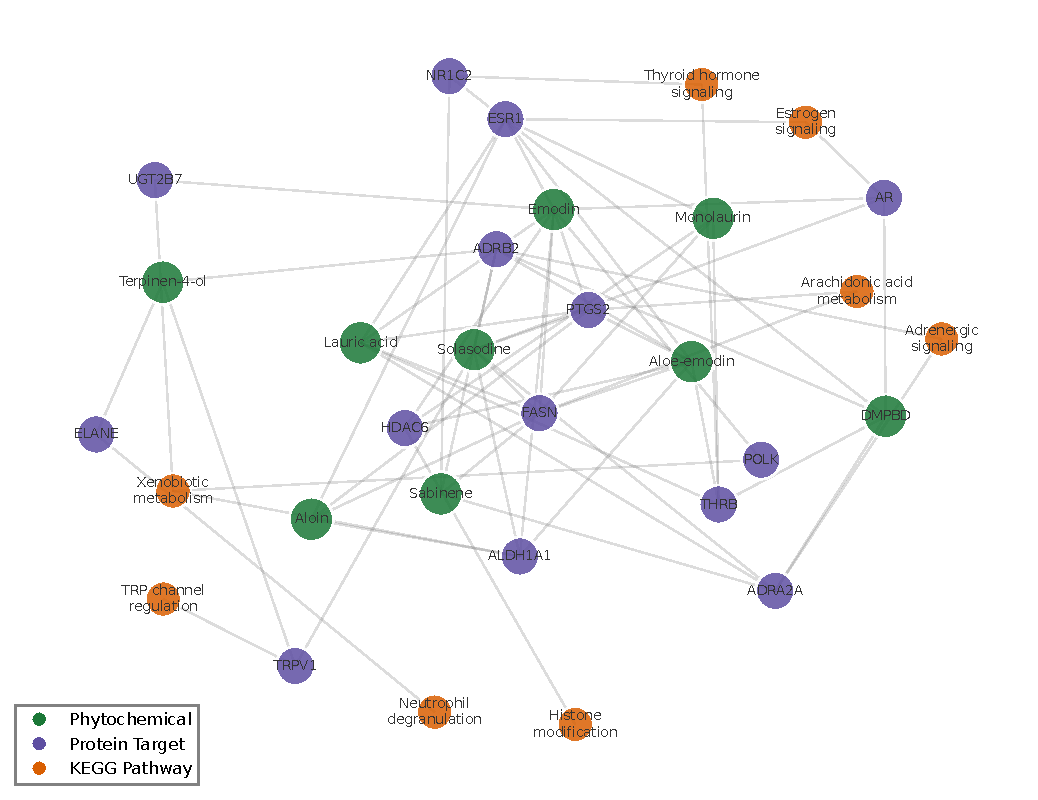
\includegraphics[width=\textwidth]{Figure_3.pdf}
\caption{Network visualization of phytochemical--target--pathway interactions related to asthma.}
\label{fig:network}
\end{figure}


\subsection{Docking results and dataset construction}

All nine phytochemical ligands (Table~\ref{tab:ligands}) were prepared for molecular docking. Ligand and protein structures were processed according to the protocols in Sections~2.6.1 and~2.6.2. Standardized PubChem CIDs and canonical SMILES ensure reproducibility of the defined chemical space, facilitating consistent comparison between sequential and HPC-accelerated workflows.

Of the 14~prioritized protein targets, 12 had available crystal structures with resolution $<$~3.0~\AA{}. Homology models were constructed for NR1C2 and ELANE, as no suitable experimental structures were available for these targets. High-resolution structures ($<$~3.0~\AA{}) are critical in molecular docking because they influence correct prediction of side-chain orientations and active-site geometries, thereby affecting binding affinity accuracy \cite{flachsenberg2023,barcelos2022}. For the two targets lacking experimental data, homology modeling was employed to complement the docking matrix. This is accepted practice given the biological significance of these targets, which would otherwise be excluded from the analysis \cite{barcelos2022}.

A final docking matrix was constructed with 9~ligands and 14~protein targets, yielding 126~ligand--protein docking combinations (Table~\ref{tab:docking-matrix}). This set was used for both sequential and HPC-based computational benchmarking.

\begin{table}[!ht]
\centering
\caption{Ligand dataset prepared for molecular docking (CID and SMILES).}
\label{tab:ligands}
\small
\begin{tabularx}{\textwidth}{lcp{8cm}}
\toprule
\textbf{Ligand} & \textbf{CID} & \textbf{Canonical SMILES} \\
\midrule
Aloe-emodin & 10207 & C1=CC2=C(C(=C1)O)C(=O)C3=C(C2=O)C=C(C=C3O)CO \\
Aloin        & 12305761 & C1=CC2=C(C(=C1)O)C(=O)C3=C({[}@H{]}2...)C=C(C=C3O)CO \\
Emodin       & 3220    & CC1=CC2=C(C(=C1)O)C(=O)C3=C(C2=O)C=C(C=C3O)O \\
Lauric acid  & 3893    & CCCCCCCCCCCC(=O)O \\
Monolaurin   & 14871   & CCCCCCCCCCCC(=O)OCC(CO)O \\
Solasodine   & 442985  & C{[}C@@H{]}1CCC@@{]}2(...) \\
DMPBD        & 96364977 & C{[}C@@H{]}(/C=C/C1=CC(=C(C=C1)OC)OC)O \\
Sabinene     & 18818   & CC(C)C12CCC(=C)C1C2 \\
Terpinen-4-ol & 11230  & CC1=CCC(CC1)(C(C)C)O \\
\bottomrule
\end{tabularx}
\end{table}

\begin{table}[!ht]
\centering
\caption{Summary of ligand and protein preparation for molecular docking.}
\label{tab:docking-matrix}
\begin{tabular}{llc}
\toprule
\textbf{Category} & \textbf{Description} & \textbf{Count / Range} \\
\midrule
Ligands        & Phytochemicals in PDBQT format               & 9 \\
Proteins       & Total prioritized targets                     & 14 \\
               & -- with crystal structures ($\leq$~3.0~\AA{})   & 12 \\
               & -- homology models (NR1C2, ELANE)             & 2 \\
Resolution     & PDB crystal structures                        & 1.5--3.0~\AA{} \\
Docking pairs  & Total ligand--protein combinations            & 126 \\
\bottomrule
\end{tabular}
\end{table}


\subsection{Computational performance benchmarking}

The computational benchmarking focused on the docking execution phase, which constitutes the dominant workload component. In sequential mode, the docking phase required \SI{29520}{s} (\SI{8.2}{hours}), while the HPC-accelerated workflow completed the same 126~ligand--protein docking tasks in \SI{255}{s} (\SI{4.25}{min}), yielding a 118.59-fold reduction in docking wall-clock time. The total end-to-end pipeline time, including data preparation ($\sim$\SI{5}{min} for both modes) and result aggregation (\SI{5}{min} sequential; \SI{40}{s} HPC), was \SI{8.4}{hours} for the sequential workflow and approximately \SI{10}{min} for the HPC workflow. It should be noted that the sequential baseline was executed on a standard workstation rather than a single LANTA core; the reported speedup therefore reflects both hardware differences and parallelization gains. As shown in Figure~\ref{fig:performance}A, the docking simulation dominated the total runtime in both modes. Docking throughput increased from 15 to 1,779~jobs/hour (Figure~\ref{fig:performance}B), yielding a parallel efficiency of \SI{94.12}{\percent} for the docking phase. This demonstrates near-linear scalability with minimal overhead, indicating effective workload distribution through SLURM's scheduling system \cite{curia2024,simakov2018}.

\begin{figure}[!ht]
\centering
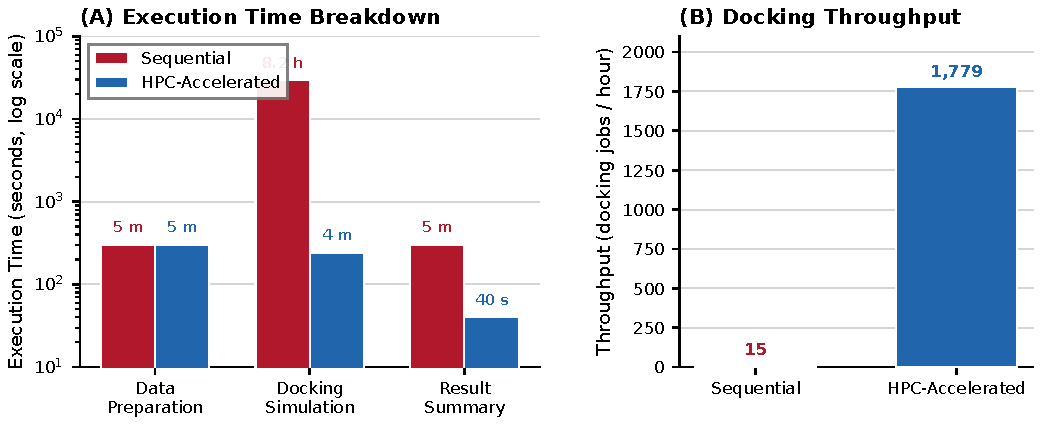
\includegraphics[width=\textwidth]{Figure_4.pdf}
\caption{Performance comparison between sequential and HPC-accelerated (LANTA) parallel workflows.}
\label{fig:performance}
\end{figure}

Numerical consistency validation demonstrated that acceleration did not compromise reproducibility (Figure~\ref{fig:validation}). Absolute differences in docking scores did not exceed \SI{0.003}{kcal/mol}, with a mean difference of $10^{-3}$~\si{kcal/mol} (Pearson $r = 0.9974$). These differences fall within the expected variability of floating-point precision calculations, which is consistent with previously reported cross-architecture differences in AutoDock Vina \cite{pham2022,tang2022}. Importantly, ligand rankings were preserved. These results indicate that the SLURM-based orchestration provides algorithmic stability while accelerating computations.

Our findings are consistent with previous HPC-based docking studies reporting speedups in the range of 20--60$\times$ \cite{kotev2023}. Tang et al.\ showed that Vina-GPU achieved an average 21-fold and maximum 50-fold acceleration compared with AutoDock Vina while maintaining accuracy \cite{tang2022}. The CPU-based SLURM job array approach in this work achieved a 118-fold practical acceleration comparing a standard workstation baseline to HPC parallel execution. While direct comparison with GPU-based methods is not possible due to differing baselines, these results demonstrate that CPU-based task parallelism via SLURM job arrays offers a practical and accessible alternative for embarrassingly parallel docking workloads. The performance and scalability results align with the paradigm shift toward ultralarge-scale virtual screening (ULVS). As stated by Gorgulla (2023), the growth of available chemical libraries to billions of compounds has made traditional sequential docking computationally unfeasible \cite{gorgulla2023}. The 118.59-fold speedup achieved on LANTA demonstrates near-linear scaling behavior, a prerequisite for modern structure-based virtual screening (SBVS) \cite{falbo2026}. This efficiency enables exploration of larger chemical space within practical timeframes, which is vital for identifying potent compounds from multi-ingredient traditional medicine formulations \cite{sadybekov2023}.

\begin{figure}[!ht]
\centering
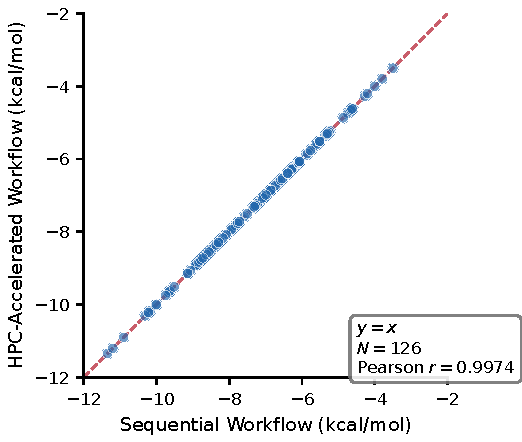
\includegraphics[width=0.65\textwidth]{Figure_5.pdf}
\caption{Numerical consistency validation of sequential and HPC-accelerated workflows.}
\label{fig:validation}
\end{figure}


\subsection{Scalability projection analysis}

To evaluate scalability beyond the benchmarked configuration (1~node, 126~cores), runtime projections were calculated with baseline throughput of 1,779~docking~jobs/hour and parallel efficiency of \SI{94.12}{\percent}. Three scenarios were considered: (i)~sequential execution, (ii)~HPC on 1~node, and (iii)~HPC on 10~nodes (1,260~cores).

For 126~docking pairs, sequential execution, HPC on 1~node, and HPC on 10~nodes required 8.4, 0.071, and \SI{0.007}{hours}, respectively (Figure~\ref{fig:scalability}). At $10^4$~docking pairs, the runtimes were approximately 667, 5.62, and \SI{0.56}{hours}. At HTS scale ($10^6$~pairs), sequential execution would require approximately 66,667~hours ($\sim$7.6~years), while HPC on 1~node and 10~nodes would require approximately 562~hours ($\sim$23~days) and 56.2~hours ($\sim$2.3~days), respectively.

These projections are based on the following engineering assumptions: (i)~steady-state parallel efficiency of 0.941, (ii)~homogeneous processing demands per docking pair, and (iii)~consistent I/O and network performance at larger workloads. Real-world efficiency at extreme scales may be lower due to filesystem contention or scheduler overhead, but these projections provide a conservative, data-driven throughput estimate. Under linear scaling assumptions, wall-clock time decreases proportionally with available cores, demonstrating that the proposed HPC workflow can extend from small-scale phytochemical datasets to HTS-scale docking. This scalability arises from the embarrassingly parallel nature of molecular docking, where each ligand--receptor pair can be evaluated independently \cite{darme2021}. SLURM job arrays distribute independent tasks without inter-process communication, minimizing scheduler and I/O overhead \cite{curia2024,simakov2018}. This scaling potential is consistent with other large-scale docking efforts, including the VirtualFlow framework, which demonstrated that distribution of independent docking jobs across large clusters can transform ultra-large library screening from impractical to routine \cite{gorgulla2020,lyu2019,eisenhuth2025}.

Numerical reliability must be maintained as computational scale increases. The high Pearson correlation ($r = 0.9974$) indicates minimal cross-platform deviations, confirming that the HPC workflow preserves numerical fidelity while scaling computational throughput \cite{lyu2019}.

\begin{figure}[!ht]
\centering
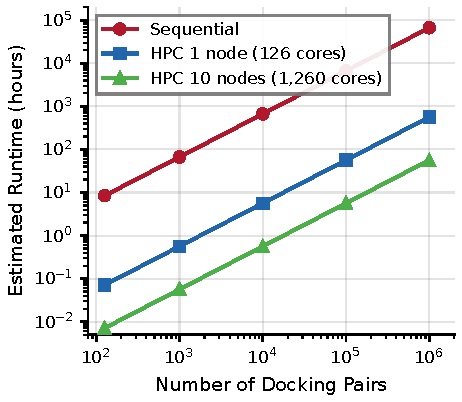
\includegraphics[width=0.65\textwidth]{Figure_6.pdf}
\caption{Scalability projection based on measured baseline throughput.}
\label{fig:scalability}
\end{figure}


\subsection{Application case study: binding affinity profile}

To validate the applicability of the HPC-based workflow, binding affinity profiles were evaluated for the 14~prioritized asthma-related protein targets. All 126~ligand--protein interactions were computed and presented in a heatmap (Figure~\ref{fig:heatmap}).

Among the screened phytochemicals, solasodine exhibited the strongest binding profile, with significant affinities toward PTGS2 ($-$\SI{11.2}{kcal/mol}) and ALDH1A1 ($-$\SI{10.0}{kcal/mol}). Representative docking poses are shown in Figure~\ref{fig:poses}. PTGS2 (COX-2) is a key inflammatory enzyme and well-established therapeutic target. Overexpression of PTGS2 is associated with increased inflammatory cell recruitment and bronchial hyperresponsiveness in the airway epithelium during asthma \cite{habib2022,barnes2022,chung2022}. The strong predicted binding between solasodine and PTGS2 is consistent with previous reports on the anti-inflammatory properties of \textit{Solanum xanthocarpum}, which may involve modulation of inflammatory enzymatic pathways \cite{firdaus2025,konar2022}.

Solasodine also exhibited high predicted binding affinity toward ALDH1A1, an enzyme associated with detoxification of lipid peroxidation products during oxidative stress in asthmatic airways \cite{hu2023}. To our knowledge, this interaction has not been previously reported in the computational or experimental literature, suggesting it may warrant further experimental investigation.

Other phytochemicals such as aloin and aloe-emodin demonstrated binding affinities in the range of $-$8 to $-$\SI{9}{kcal/mol} against targets including PTGS2, FASN, and ALDH1A1. Monolaurin, sabinene, lauric acid, and DMPBD exhibited moderate affinities ($-$7.5 to $-$\SI{7.0}{kcal/mol}) against THRB, ADRA2A, and AR. This convergent binding pattern toward different inflammatory mediators supports a multi-target interaction architecture \cite{li2025}. The distributed interaction pattern is consistent with polypharmacology, where therapeutic effects arise from modulation of multiple molecular nodes rather than selective inhibition of a single enzyme \cite{noor2022,yang2025,joshi2025}. Such system-level interaction patterns are relevant to asthma, a heterogeneous disease involving immune dysregulation, epithelial remodeling, neurogenic inflammation, and metabolic reprogramming \cite{habib2022,barnes2022,chung2022}.

\begin{figure}[!ht]
\centering
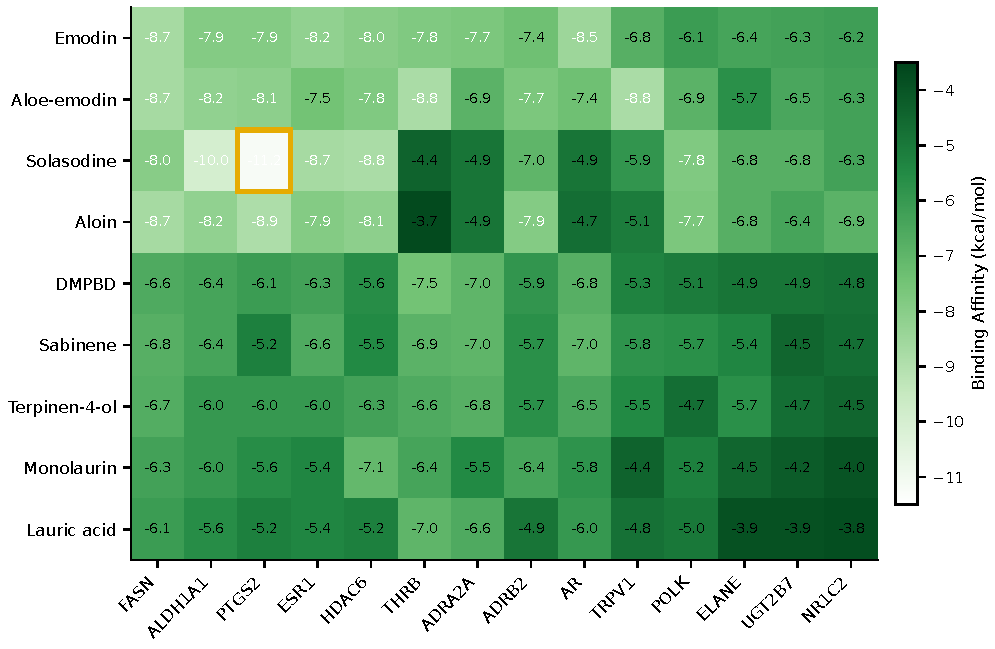
\includegraphics[width=\textwidth]{Figure_7.pdf}
\caption{Heatmap of binding affinity scores for all phytochemical--receptor pairs.}
\label{fig:heatmap}
\end{figure}

\begin{figure}[!ht]
\centering
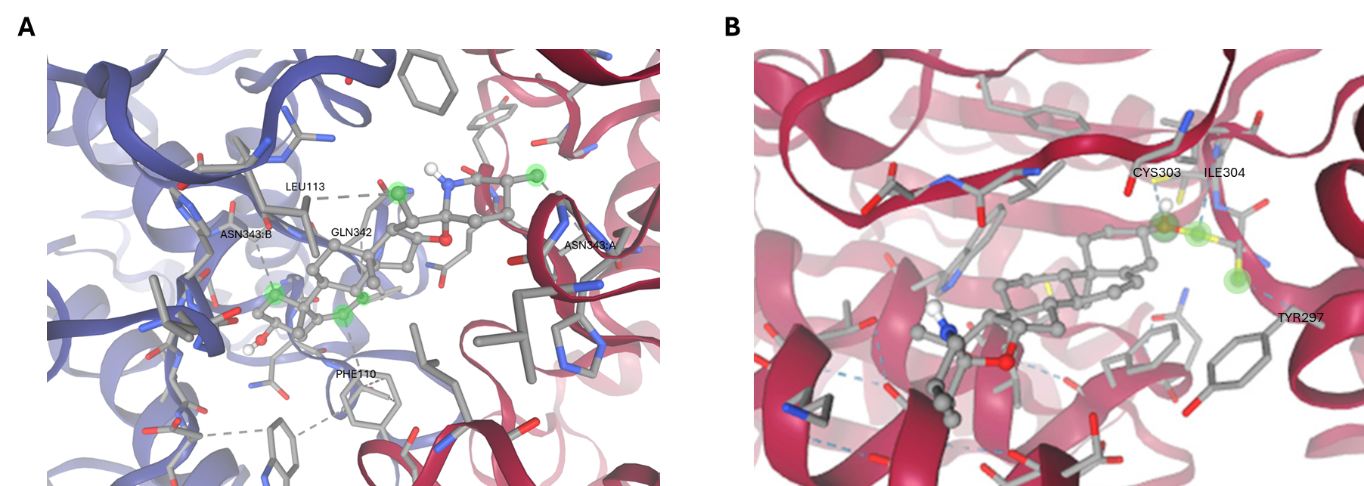
\includegraphics[width=\textwidth]{fig8_docking_poses.png}
\caption{Docking poses of (A) solasodine--PTGS2 and (B) solasodine--ALDH1A1.}
\label{fig:poses}
\end{figure}

For contextual benchmarking, standard drugs were docked under identical conditions (Figure~\ref{fig:drug-comparison}). Dexamethasone demonstrated a binding affinity of $-$\SI{9.2}{kcal/mol} to PTGS2, while salbutamol showed $-$\SI{8.1}{kcal/mol} to ADRB2. Notably, solasodine exhibited a stronger predicted binding to PTGS2 than dexamethasone. Although docking scores do not directly reflect pharmacodynamic potency, they indicate computational plausibility of phytochemical engagement with clinically relevant targets. Because identical preprocessing, grid parameters, and scoring functions were applied to all ligands, cross-compound comparisons remain methodologically consistent.

\begin{figure}[!ht]
\centering
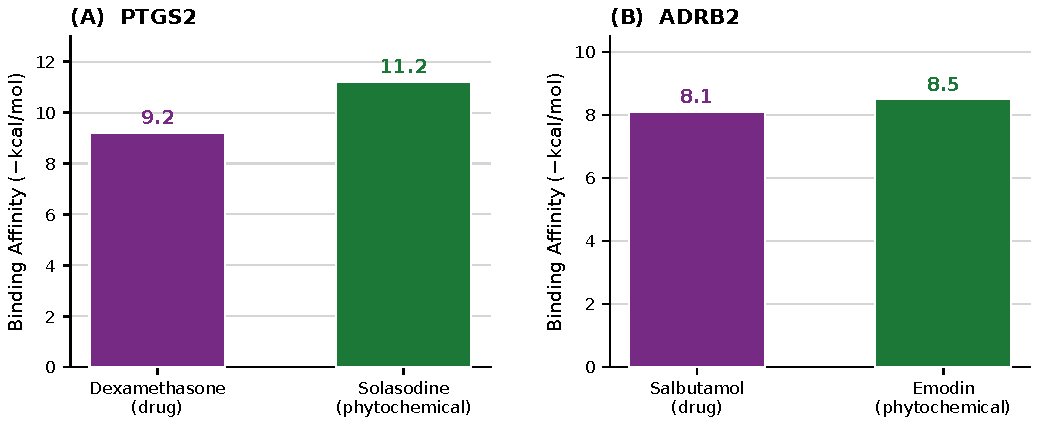
\includegraphics[width=\textwidth]{Figure_9.pdf}
\caption{Comparative binding affinities of lead phytochemicals and standard controls for asthma-related targets.}
\label{fig:drug-comparison}
\end{figure}

The selection of tools and resources ensured reproducibility and integration into the HPC workflow. Compound and protein data were obtained from internationally recognized sources (PubChem, KEGG, PDB), ensuring accuracy and reproducibility \cite{flachsenberg2023,azevedo2024,li2025b}. RDKit, Open Babel, and Conda provided well-documented, open-source cheminformatics capabilities \cite{herz2023}. SwissTargetPrediction, a frequently cited web server, generated preliminary hypotheses on protein--ligand interactions \cite{daina2019}. Custom Python and Bash scripts automated the integration of all workflow components. AutoDock Vina was selected as the docking engine for its extensive validation record and established balance between computational efficiency and predictive accuracy \cite{seeliger2010,ivanova2022}.

The automated HPC-enabled workflow demonstrated both computational acceleration and structured prioritization of multi-target interaction profiles within a reproducible framework.


% ============================================================
% 4. CONCLUSION
% ============================================================
\section{Conclusion}

This research presented an HPC-accelerated automated workflow for evaluation of phytochemical--target interactions in a Thai traditional anti-asthma herbal formulation. Through automated compound mining and target filtering, the workflow reduced predicted interactions from 197 to 14 biologically prioritized protein targets, achieving a data reduction ratio of \SI{92.9}{\percent}. Performance benchmarking demonstrated significant acceleration on the LANTA supercomputer: the execution time for 126~docking pairs decreased from \SI{8.4}{hours} (sequential, workstation) to \SI{4.25}{min} (HPC, parallel), representing a 118-fold practical reduction in wall-clock time and increasing throughput from 15 to 1,779~docking~jobs/hour. Parallel efficiency of \SI{94.12}{\percent} indicated near-linear scalability using SLURM job array orchestration. Numerical validation ($r = 0.9974$) demonstrated that acceleration did not compromise reproducibility within floating-point precision limits. Scalability projections supported feasibility for expansion to HTS-scale datasets ($10^6$~docking pairs) with multi-node allocation, although real-world performance at extreme scales may be influenced by filesystem constraints or scheduler contention.

Several limitations should be acknowledged. First, no re-docking validation was performed to assess the reliability of the docking protocol; future work should include re-docking of co-crystallized ligands with RMSD evaluation. Docking scores were computed using AutoDock Vina~1.1.2, selected for its extensive validation record and compatibility with the automated workflow; however, newer versions (1.2.x) offer improved scoring functions. Scores were based on predicted binding affinity under rigid receptor assumptions and did not incorporate protein flexibility or solvation effects. Homology modeling of two targets (NR1C2, ELANE) may introduce additional structural uncertainty. All in-silico predictions require experimental validation before translational conclusions can be drawn.

The case study demonstrated that the HPC workflow not only improved computational speed but also enabled structured prioritization of multi-target interaction profiles. Binding affinity patterns supported a network-oriented, polypharmacological approach, providing a rational computational basis for further experimental validation.

The proposed HPC workflow represents a scalable, reproducible, and computationally efficient approach to natural product-based virtual screening. Its architecture is potentially adaptable to larger compound libraries, molecular dynamics simulations, and AI-based scoring methods, establishing it as a platform for next-generation computational ethnopharmacology and drug discovery research.

Future work should address the current limitations through re-docking validation of the docking protocol, integration of molecular dynamics simulations for binding pose refinement, and experimental validation of the top-ranked phytochemical--target interactions. Extension of the workflow to GPU-accelerated docking engines and AI-based scoring functions would further enhance throughput and predictive accuracy.


% ============================================================
% ACKNOWLEDGMENTS
% ============================================================
\section*{Acknowledgments}

This research was primarily supported by the HPC-IGNITE project, which provided fundamental opportunities, education, and mentorship. We express sincere gratitude to the Lampang Chamber of Commerce, the National Research Council of Thailand (NRCT), the Association for Computing Machinery (ACM), Amazon Web Services (AWS), the Ministry of Higher Education, Science, Research and Innovation, Thammasat University, and the NSTDA Supercomputer Center (ThaiSC).

We thank the NSTDA Supercomputer Center (ThaiSC) for providing access to the LANTA supercomputer system, without which this research would not have been possible.


% ============================================================
% ETHICS, COI, DATA
% ============================================================
\section*{Ethics Statement}

This research did not involve human participants or animal subjects; therefore, ethical approval was not required.

\section*{Conflicts of Interest}

The authors declare no conflicts of interest.

\section*{Data Availability}

All data generated or analyzed during this study are included in this article.


% ============================================================
% REFERENCES
% ============================================================
\begingroup
\small
\begin{thebibliography}{57}

\bibitem{jeyasingh2024}
J.~R. Jeyasingh, J.~I. Glory,
\textit{Biosci.\ Biotechnol.\ Res.\ Asia} \textbf{2024}, \textit{21}(1), 11.

\bibitem{babalola2025}
O.~O. Babalola, K.~Bridget, G.~Oyubu, et al.,
\textit{Discov.\ Chem.} \textbf{2025}, \textit{2}(1), 297.

\bibitem{gina2023}
Global Initiative for Asthma,
Global Strategy for Asthma Management and Prevention, \textbf{2023}.

\bibitem{vos2020}
T.~Vos, S.~S. Lim, C.~Abbafati, et al.,
\textit{Lancet} \textbf{2020}, \textit{396}(10258), 1204.

\bibitem{siddiqui2025}
B.~Siddiqui, C.~S. Yadav, M.~Akil, et al.,
\textit{Comb.\ Chem.\ High Throughput Screen.} \textbf{2025}.

\bibitem{gupta2024}
P.~Gupta, A.~Chanana, Y.~R. Kulkarni, et al.,
\textit{Curr.\ Artif.\ Intell.} \textbf{2024}, \textit{2}(1).

\bibitem{roy2024}
R.~B. Roy, D.~Tiwari,
\textit{Proc.\ ACM Meas.\ Anal.\ Comput.\ Syst.} \textbf{2024}, \textit{8}(1), 1.

\bibitem{gorgulla2020}
C.~Gorgulla, A.~Boeszoermenyi, Z.~F. Wang, et al.,
\textit{Nature} \textbf{2020}, \textit{580}(7805), 663.

\bibitem{gorgulla2023}
C.~Gorgulla,
\textit{Annu.\ Rev.\ Biomed.\ Data Sci.} \textbf{2023}, \textit{6}(1), 229.

\bibitem{chowdhury2020}
F.~Chowdhury, Y.~Zhu, F.~Di Natale, et al.,
in \textit{Proc.\ Fifth Int.\ Parallel Data Syst.\ Workshop (PDSW)}, IEEE, \textbf{2020}, 34.

\bibitem{varavithya2023}
V.~Varavithya, S.~Prueksaaroon,
\textit{ECTI Trans.\ Comput.\ Inf.\ Technol.} \textbf{2023}, \textit{17}(2), 255.

\bibitem{goponenko2024}
A.~V. Goponenko, B.~A. Allan, J.~M. Brandt, et al.,
in \textit{SC24-W: Workshops of SC}, \textbf{2024}, 1506.

\bibitem{awan2016}
M.~G. Awan, F.~Saeed,
\textit{Bioinformatics} \textbf{2016}, \textit{32}(10), 1518.

\bibitem{daina2019}
A.~Daina, O.~Michielin, V.~Zoete,
\textit{Nucleic Acids Res.} \textbf{2019}, \textit{47}(W1), W357.

\bibitem{hagberg2008}
A.~Hagberg, P.~J. Swart, D.~A. Schult,
in \textit{Proc.\ 7th Python in Science Conf.\ (SciPy2008)}, \textbf{2008}.

\bibitem{hunter2007}
J.~D. Hunter,
\textit{Comput.\ Sci.\ Eng.} \textbf{2007}, \textit{9}(3), 90.

\bibitem{flachsenberg2023}
F.~Flachsenberg, C.~Ehrt, T.~Gutermuth, et al.,
\textit{J.\ Chem.\ Inf.\ Model.} \textbf{2023}, \textit{64}(1), 219.

\bibitem{oboyle2011}
N.~M. O'Boyle, M.~Banck, C.~A. James, et al.,
\textit{J.\ Cheminf.} \textbf{2011}, \textit{3}(1), 33.

\bibitem{gasteiger1980}
J.~Gasteiger, M.~Marsili,
\textit{Tetrahedron} \textbf{1980}, \textit{36}(22), 3219.

\bibitem{seeliger2010}
D.~Seeliger, B.~L. de Groot,
\textit{J.\ Comput.-Aided Mol.\ Des.} \textbf{2010}, \textit{24}(5), 417.

\bibitem{jette2023}
M.~A. Jette, T.~Wickberg,
in \textit{Workshop Job Sched.\ Strat.\ Parallel Process.}, Springer, \textbf{2023}, 3.

\bibitem{amdahl1967}
G.~M. Amdahl,
in \textit{Proc.\ Spring Joint Comput.\ Conf.}, \textbf{1967}, 483.

\bibitem{eijkhout2010}
V.~Eijkhout,
\textit{Introduction to High Performance Scientific Computing}, Lulu.com, \textbf{2010}.

\bibitem{hothorn2011}
T.~Hothorn, F.~Leisch,
\textit{Brief.\ Bioinform.} \textbf{2011}, \textit{12}(3), 288.

\bibitem{habib2022}
N.~Habib, M.~A. Pasha, D.~D. Tang,
\textit{Cells} \textbf{2022}, \textit{11}(17), 2764.

\bibitem{liu2026}
Z.~Liu, H.~Zhang, B.~Wan, et al.,
\textit{Drug Des.\ Dev.\ Ther.} \textbf{2026}, 1.

\bibitem{slob2018}
E.~M. Slob, S.~J. Vijverberg, C.~N. Palmer, et al.,
\textit{Pediatr.\ Allergy Immunol.} \textbf{2018}, \textit{29}(7), 705.

\bibitem{tanaka2024}
M.~Tanaka, K.~Shirakura, Y.~Takayama, et al.,
\textit{Commun.\ Biol.} \textbf{2024}, \textit{7}(1), 599.

\bibitem{potaczek2024}
D.~P. Potaczek, S.~Bazan-Socha, E.~Wypasek, et al.,
\textit{Int.\ Arch.\ Allergy Immunol.} \textbf{2024}, \textit{185}(7), 641.

\bibitem{ito2025}
A.~Ito,
\textit{Endocr.\ J.} \textbf{2025}, \textit{72}(9), 979.

\bibitem{manti2024}
S.~Manti, A.~Gambadauro, F.~Galletta, et al.,
\textit{Int.\ J.\ Mol.\ Sci.} \textbf{2024}, \textit{25}(19), 10234.

\bibitem{kotev2023}
M.~Kotev, C.~Diaz Gonzalez,
in \textit{HPC for Drug Discovery and Biomedicine}, Springer, \textbf{2023}, 265.

\bibitem{noor2022}
F.~Noor, M.~Tahir ul Qamar, U.~A. Ashfaq, et al.,
\textit{Pharmaceuticals} \textbf{2022}, \textit{15}(5), 572.

\bibitem{yang2025}
L.~Yang, H.~Wang, Z.~Zhu, et al.,
\textit{Pharmaceuticals} \textbf{2025}, \textit{18}(7), 1074.

\bibitem{barcelos2022}
M.~P. Barcelos, S.~Q. Gomes, L.~B. Federico, et al.,
in \textit{Res.\ Topics Bioact.\ Environ.\ Energy}, Springer, \textbf{2022}, 481.

\bibitem{curia2024}
N.~E. Curia-Alcantara, C.~Inga-Cove\~{n}as, W.~Auccahuasi,
in \textit{Proc.\ 3rd Int.\ Conf.\ Autom.\ Comput.\ Renew.\ Syst.\ (ICACRS)}, IEEE, \textbf{2024}, 771.

\bibitem{simakov2018}
N.~A. Simakov, R.~L. DeLeon, M.~D. Innus, et al.,
in \textit{Proc.\ Pract.\ Exp.\ Adv.\ Res.\ Comput.}, \textbf{2018}, 1.

\bibitem{pham2022}
T.~N.~H. Pham, T.~H. Nguyen, N.~M. Tam, et al.,
\textit{J.\ Comput.\ Chem.} \textbf{2022}, \textit{43}(3), 160.

\bibitem{tang2022}
S.~Tang, R.~Chen, M.~Lin, et al.,
\textit{Molecules} \textbf{2022}, \textit{27}(9), 3041.

\bibitem{falbo2026}
E.~Falbo, P.~Delre, C.~Cerchia, et al.,
in \textit{Applied AI for Drug Discovery}, Springer, \textbf{2026}, 105.

\bibitem{sadybekov2023}
A.~V. Sadybekov, V.~Katritch,
\textit{Nature} \textbf{2023}, \textit{616}(7958), 673.

\bibitem{darme2021}
P.~Darme, M.~Dauchez, A.~Renard, et al.,
\textit{Int.\ J.\ Mol.\ Sci.} \textbf{2021}, \textit{22}(14), 7489.

\bibitem{lyu2019}
J.~Lyu, S.~Wang, T.~E. Balius, et al.,
\textit{Nature} \textbf{2019}, \textit{566}(7743), 224.

\bibitem{eisenhuth2025}
P.~Eisenhuth, F.~Liessmann, R.~Moretti, et al.,
\textit{Commun.\ Chem.} \textbf{2025}, \textit{8}(1), 335.

\bibitem{barnes2022}
M.~V. Barnes, P.~J. Openshaw, R.~S. Thwaites,
\textit{Cells} \textbf{2022}, \textit{11}(7), 1153.

\bibitem{chung2022}
K.~F. Chung, P.~Dixey, H.~Abubakar-Waziri, et al.,
\textit{Chin.\ Med.\ J.} \textbf{2022}, \textit{135}(10), 1141.

\bibitem{firdaus2025}
A.~Firdaus, M.~H. Yunus, S.~K. Izhar, et al.,
\textit{Recent Pat.\ Biotechnol.} \textbf{2025}, \textit{19}(1), 2.

\bibitem{konar2022}
A.~Konar, R.~Chatterjee,
\textit{Int.\ J.\ Sci.\ Res.\ Biol.\ Sci.} \textbf{2022}, \textit{9}(5), 196.

\bibitem{hu2023}
X.~T. Hu, B.~W. Chen, Y.~J. Cao, et al.,
\textit{World J.\ Otorhinolaryngol.\ Head Neck Surg.} \textbf{2023}, \textit{9}(4), 320.

\bibitem{li2025}
Y.~Li, X.~Liu, J.~Zhou, et al.,
\textit{Front.\ Pharmacol.} \textbf{2025}, \textit{16}, 1541509.

\bibitem{joshi2025}
C.~P. Joshi, A.~Baldi, N.~Kumar, et al.,
\textit{Naunyn-Schmiedeberg's Arch.\ Pharmacol.} \textbf{2025}, \textit{398}(5), 4689.

\bibitem{azevedo2024}
D.~Q. de Azevedo, B.~M. Campioni, F.~A. Pedroz Lima, et al.,
\textit{Future Med.\ Chem.} \textbf{2024}, \textit{16}(10), 1029.

\bibitem{li2025b}
X.~L. Li, J.~Q. Zhang, X.~J. Shen, et al.,
\textit{Acta Pharmacol.\ Sin.} \textbf{2025}, \textit{46}(2), 235.

\bibitem{herz2023}
A.~M. Herz, T.~Kellici, I.~Morao, et al.,
in \textit{HPC for Drug Discovery and Biomedicine}, Springer, \textbf{2023}, 241.

\bibitem{ivanova2022}
L.~Ivanova, M.~Karelson,
\textit{Molecules} \textbf{2022}, \textit{27}(24), 9041.

\bibitem{kumar2024}
N.~Kumar, K.~Saluja, V.~Mehta, et al.,
in \textit{Computational Biology in Drug Discovery and Repurposing}, Apple Academic Press, \textbf{2024}, 75.

\end{thebibliography}
\endgroup

\end{document}
